\label{sec:smartcontract}

We implement a smart contract that can (1) verify whether a solution is feasible and (2) compute the value of the objective function for a feasible solution.
Compared to finding an optimal solution, these operations are computationally inexpensive, and they can easily be performed on a blockchain-based decentralized platform. Thus, we implement a smart contract that provides the following functionality:
\begin{itemize}
\item Solutions may be submitted to the contract at any time during the solving phase. 
The contract verifies the feasibility of each submitted solution, and if the solution is feasible, then it computes the value of the objective function.
The contract always keeps track of the best feasible solution submitted so far, which we call the \emph{candidate solution}.
\item At the end of the solving phase, the contract finalizes resource assignments for the cycle based on the candidate solution. If no solution has been submitted to the contract, then an empty allocation is used as a solution, which is always feasible but attains zero objective. % which might be the case right after the trading system has been launched then the finalization event does not return any solution.
%\item Upon finalization, the contract must notify providers and consumers about finalized assignments. 
%This can be done using the event filter mechanisms provided by blockchains like Ethereuem. \cite{ref}.
\end{itemize}

This simple functionality achieves a high level of security and reliability.
Firstly, it is clear that an adversary cannot force the contract to finalize assignments based on an incorrect (i.e., infeasible) solution since such a solution would be rejected.
Similarly, an adversary cannot force the contract to choose an inferior solution instead of a superior one.
In sum, the only action available to the adversary is proposing a superior feasible solution, which would actually improve the transactive management platform.

%\Aron{This paragraph should be omitted (and included in the Industrial Informatics paper).}
%The contract is also reliable and can tolerate temporary disruptions in the solver or the communication network. As the sets of offers can only grow over time, the contract can use a candidate solution submitted during time interval $t$ to finalize assignments in any subsequent time interval $\tau > t$.
%In fact, without receiving new solutions, the difference between the amount of finalized assignments and the optimum will increase only gradually:
%since the earlier candidate solution can specify assignments for any future time interval,
%the difference is only due to the offers that have been posted since the solution was found and submitted.

%\subsection{Correct-by-Construction Design of the Smart Contract}
To ensure that the smart-contract code is correct-by-construction~\cite{sifakis2013RSD}, we use the formal design environment FSolidM~\cite{mavridou2018designing} to design and generate the Solidity code of the smart contract. FSolidM allows designing Ethereum smart contracts as Labelled Transition Systems (LTS) with formal semantics. Each LTS can then be given to the NuSMV model checker~\cite{cimatti2002nusmv} to verify liveness, deadlock-freedom, and safety properties, which can capture important security concerns. % and vulnerabilities. 


\begin{figure}[t]
\centering
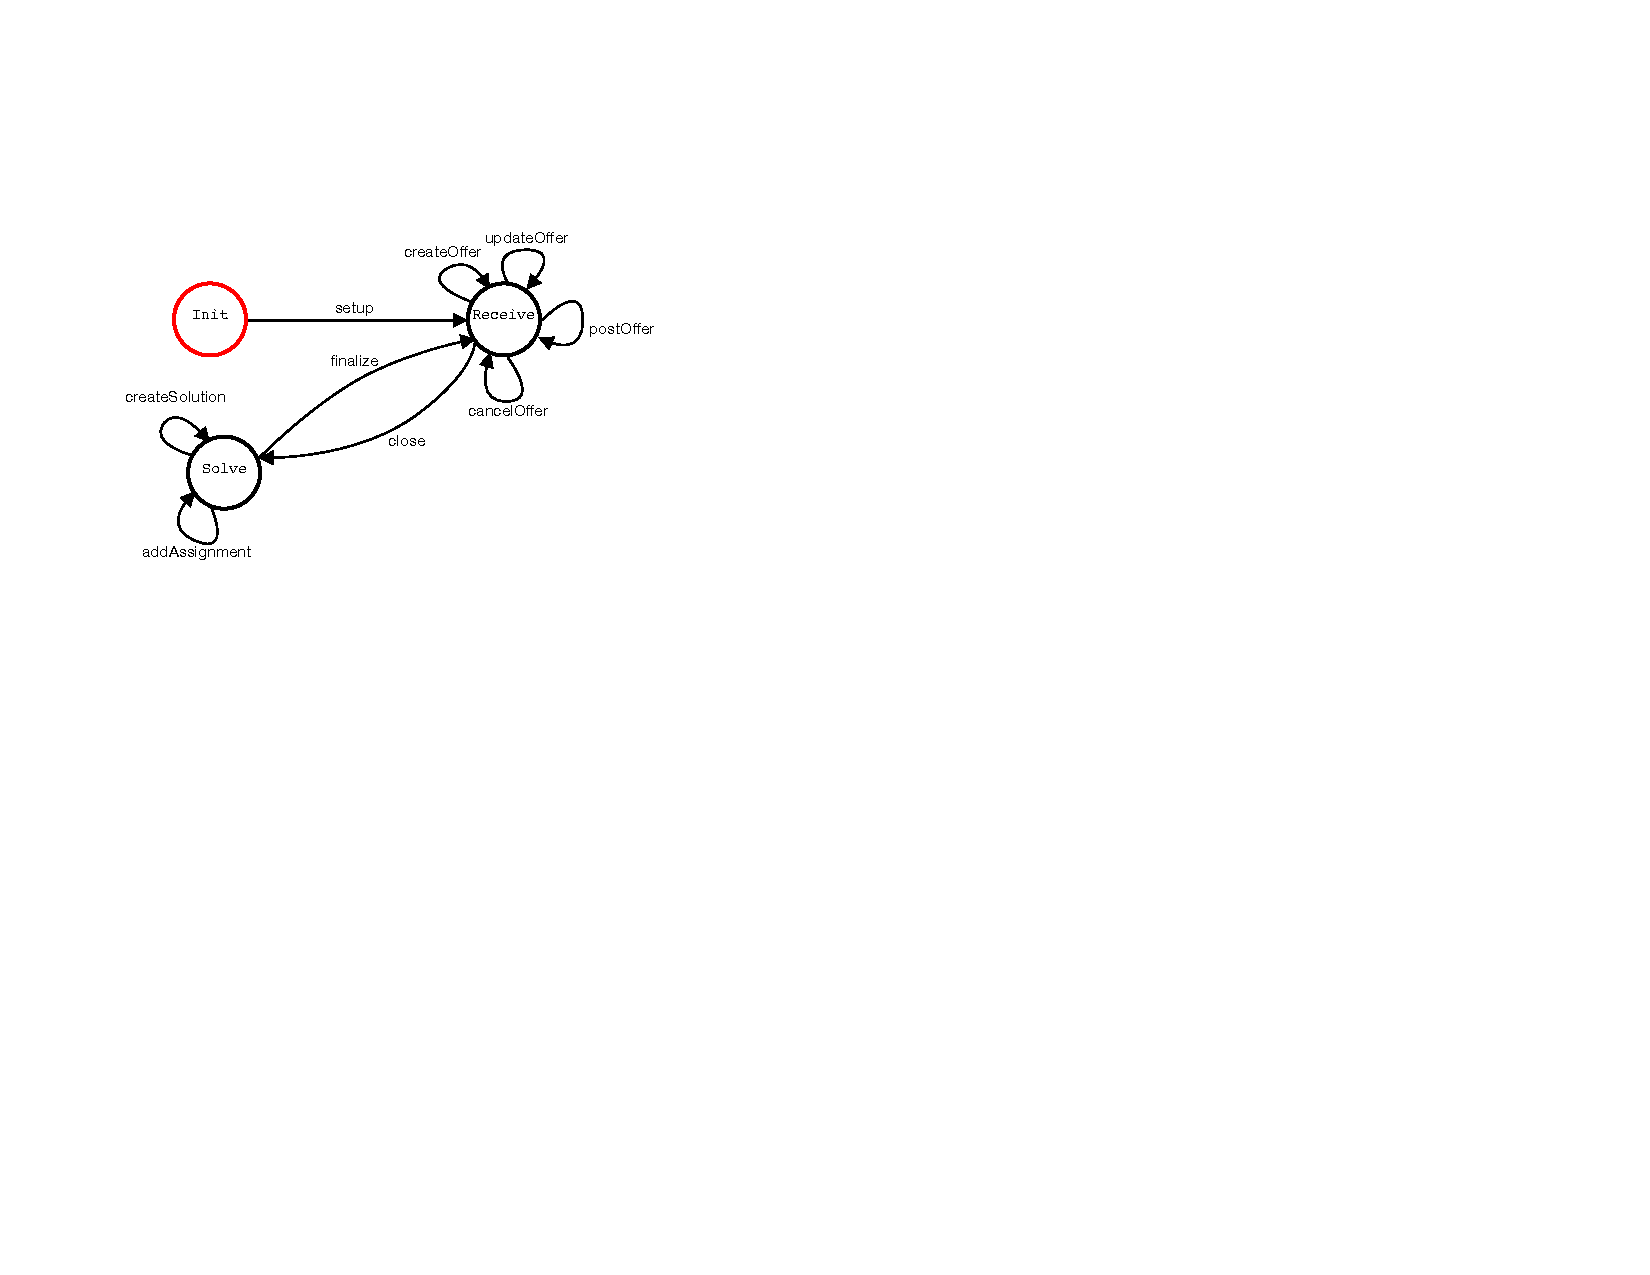
\includegraphics[width=0.8\columnwidth]{ResourceAllocationFSM.pdf}
\caption{FSolidM model of the \Platform smart contract.}
\label{fig:FSM}
\end{figure}

%\ad{Aron - please explain all the states of the smart contract here. The state machine diagram should be updated as well. please describe the mapping structure - how types are mapped in the smart contract here as well.}
%\Aron{What do you mean by mapping structure?}
%\Anastasia{I have updated the LTS figure and the description. }

In Figure~\ref{fig:FSM}, we present the LTS representation of the transactive-platform smart contract, designed with FSolidM. The contract has three states:\footnote{Generated smart-contract code is not included in the paper because of space constraints. However, interested readers can view the code at \texttt{\url{https://github.com/visor-vu/transaction-management-platform}}}
\begin{itemize}[noitemsep, topsep=0pt, leftmargin=1em]
    \item \texttt{Init}, in which the contract has been deployed but  not been initialized. Before the contract can be used, it must be initialized (i.e., numerical parameters must be set~up).
    \item \texttt{Receive}, which corresponds to the \emph{offering} phase of a cycle (see Section~\ref{sec:scheduling}).
    In this state, prosumers may post (or cancel) their offers.
    \item \texttt{Solve}, which corresponds to the \emph{solving} phase of a cycle (see Section~\ref{sec:scheduling}). In this state, solvers may submit solutions (i.e., resource allocations) based on the posted (but not cancelled) offers.
\end{itemize}

In FSolidM, smart-contract functions are modeled as LTS transitions. Note that by design, each function may be executed only if the contract is in the origin state of the corresponding transition.
Our smart contract  has the following transitions (after the name of each transition, we list the function parameters):
\begin{itemize}[leftmargin=1em, noitemsep]
    \item from state \texttt{Init}:
    \begin{itemize}[noitemsep, leftmargin=0.5em]
        \item \texttt{setup(uint64 numTypes, uint64 precision, uint64 maxQuantity)}: initializes a contract with numerical parameter values, setting up the number of resource types, the arithmetic precision for calculations, and the maximum quantity that may be offered; upon execution, the contract transitions to state \texttt{Receive}.
    \end{itemize}
    \item from state \texttt{Receive}:
    \begin{itemize}[noitemsep, leftmargin=0.5em]
        \item \texttt{createOffer(bool providing, uint64 misc))}: creates a blank offer (belonging to the prosumer invoking this transition) within the smart contract; parameter \texttt{providing} is true for providers and false for consumers, parameter \texttt{misc} is an arbitrary value that prosumers may use for their own purposes (e.g., to distinguish between their own offers); emits an \texttt{OfferCreated} event.
        \item \texttt{updateOffer(uint64 ID, uint64 resourceType, uint64 quantity, uint64 value)}: sets quantity and value for a resource type in an existing  offer (identified by the \texttt{ID} given in the \texttt{OfferCreated} event); may be invoked only by the entity that created the offer, and only if the offer exists but has not been posted yet; emits an \texttt{OfferUpdated} event.
        \item \texttt{postOffer(uint64 ID)}: posts an existing offer, enabling solvers to include this offer in a solution; may be invoked only by the entity that created the offer; emits an \texttt{OfferPosted} event.
        \item \texttt{cancelOffer(uint64 ID)}: cancels (i.e., ``unposts'') an offer, forbidding solvers from including this offer in a solution; may be invoked only by the entity that created the offer; emits an \texttt{OfferCanceled} event.
        \item \texttt{close()}: protected by a  guard condition on time, which prevents the execution of this transition before the offering phase of the current cycle ends; transitions to state \texttt{Solve}; emits a \texttt{Closed} event.
    \end{itemize}
    \item from state \texttt{Solve}:
    \begin{itemize}[noitemsep, leftmargin=0.5em]
        \item \texttt{createSolution(uint64 misc)}: creates a new, empty solution (i.e., resource allocation) within the smart contract; parameter \texttt{misc} is an arbitrary value that solvers may use for their own purposes (e.g., to distinguish between their own solutions); emits a \texttt{SolutionCreated} event.
        \item \texttt{addAssignment(uint64 ID, uint64 providingOfferID, uint64 consumingOfferID, uint64 resourceType, uint64 quantity, uint64 value)}: adds a resource assignment to an existing solution (identified by the \texttt{ID} given in the \texttt{SolutionCreated} event); may be invoked only by the entity that created the solution; checks a number of constraints ensuring that the solution remains valid if this assignment is added; emits an \texttt{AssignmentAdded} event.
        \item \texttt{finalize()}: selects the best solution and finalizes it by emitting an \texttt{AssignmentFinalized} event for each assignment in the solution; protected by a guard condition on time, which prevents the execution of this transition before the solving phase of the current cycle ends; transitions to state \texttt{Receive}.
    \end{itemize}
\end{itemize}
Notice that posting an offer and submitting a solution require at least three and two function calls, respectively.
The reason for dividing these operations into multiple functions is to ensure that the computational costs of these functions are constant.
Otherwise, posting a complex offer or submitting a complex solution could be infeasible due to large computational costs, which could exceed the gas limit.\footnote{In Ethereum, each transaction is allowed to consume only a limited amount of gas, which corresponds to the computational and storage cost of executing the transaction.}



% \begin{lstlisting}[language=Solidity, caption=Extract of the Generated Smart Contract. Full contract is available at \url{https://github.com/visor-vu/transaction-management-platform}. ,label={lst:finalize}]
% pragma solidity ^0.4.19;
% contract SolidWorx {     
%     function setup(...) public {
%         //setup SolidWorx to be used with a fixed type of resources. 
%     }
%     //This is the syntax of an offer.
%     struct Offer {
%         bool providing; 
%         // true: providing offer
%         // false: consumption offer
%         uint64 prosumer; 
%         bool posted;
%         mapping(uint64 => uint64) quantity;
%         mapping(uint64 => uint64) value;
%     }
%     //syntax of an Assignment
%     struct Assignment {
%         uint64 providingOfferID;
%         uint64 consumingOfferID;
%         uint64 resourceType;
%         uint64 quantity;
%         uint64 value;
%     }
%     //A solution contains many assignments.
%     struct Solution {
%         mapping(uint64 => Assignment) assignments;
%         uint64 numAssignments;
%         uint64 objective;
%         mapping(uint64 => uint256) allocated;     
%     }
%     function createOffer(bool providing, uint64 misc, uint64 prosumer) public {
%         ...
%     }
%     function updateOffer(uint64 ID, uint64 resourceType, uint64 quantity, uint64 value) public {
%         ...
%     }
%     function postOffer(uint64 ID) public {
%         ...
%     }
%     function cancelOffer(uint64 ID) public {
%         ...
%     }
%     ...
%     function createSolution(uint64 misc) public {
%         ...
%     }
%     function addAssignment(...) public {
%         ...
%     }
%     function finalize() public {
%         ...
%     }
% }
% \end{lstlisting}

%Listing \ref{lst:finalize} presents the generated API and the guards for the smart contract in \Platform. 




%\subsection{Operation Workflow }

\begin{figure}[t]
    \centering
    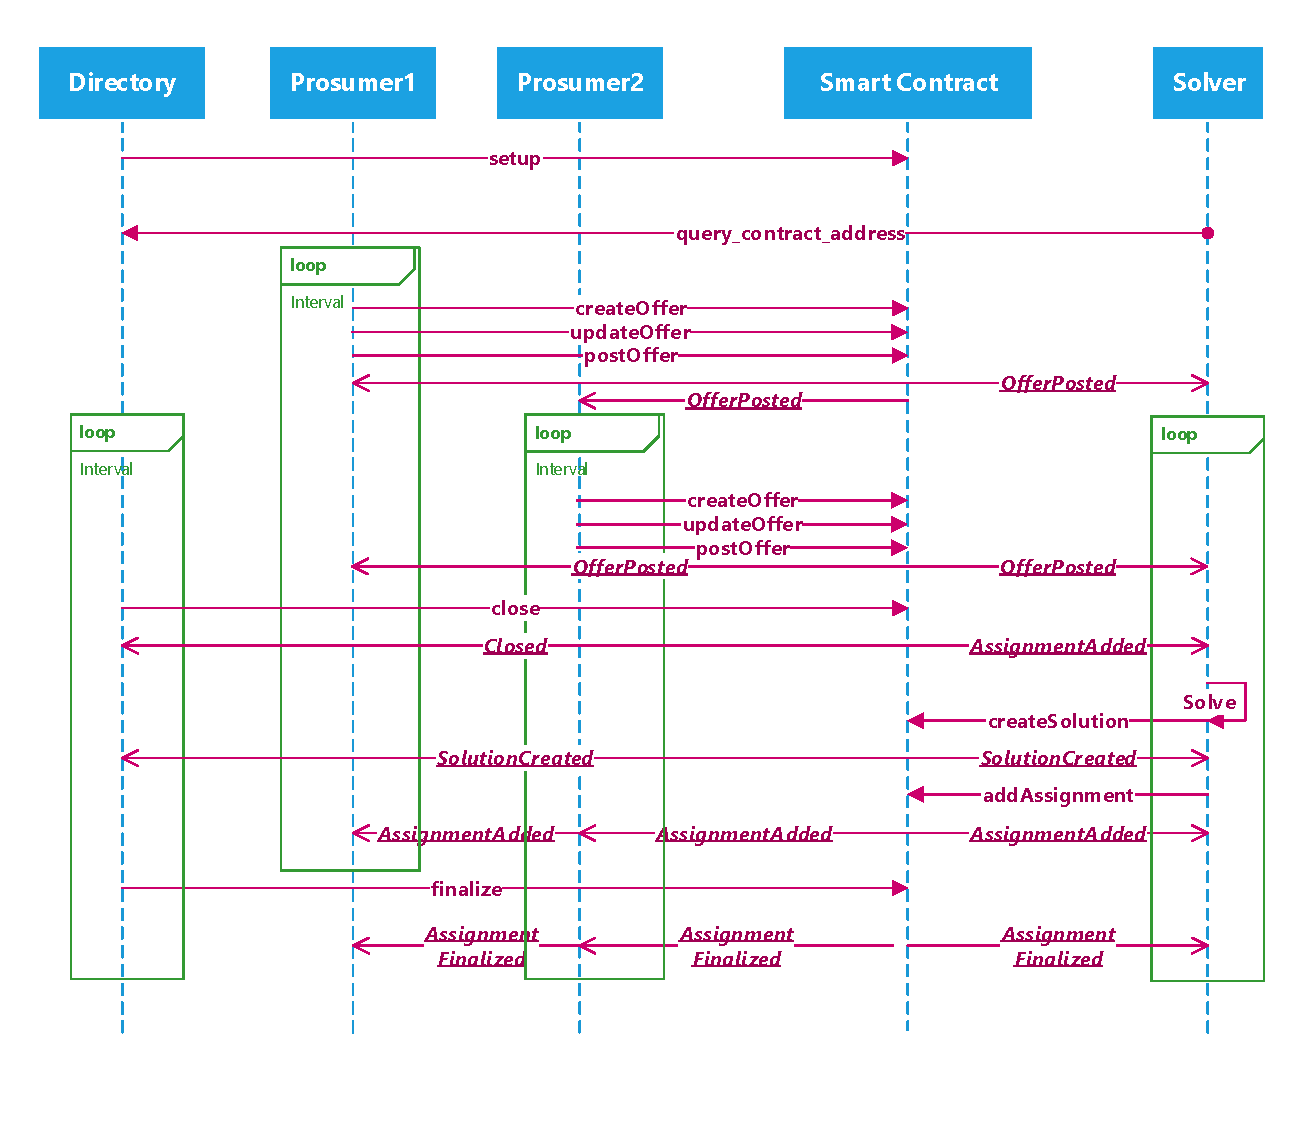
\includegraphics[width=\columnwidth]{Workflow.pdf}
    \caption{A possible sequence of operations in \Platform. Underlined text denotes events emitted by the smart contract. Some events, such as \texttt{OfferUpdated}, are omitted for simplicity. %The offers can be updated by a prosumer before they are marked as posted. 
    %See Listing \ref{lst:finalize} for the API.} % Prosumers and Solvers use the directory to find one of the miner nodes running the smart contract. They then connect to the  mining node.
    }
    \vspace{-0.1in}
    \label{fig:workflow}
\end{figure}

 A typical sequence of function calls and events in \Platform is shown in Figure \ref{fig:workflow}.
